\documentclass[11pt]{article}


%%%%%%%%%%%%%%%%%%%%%%%%%%%%%%%%%%%%%%%%%%%%%%%%%%%%%%%%%%%%%%%%%%%%%%%%%%%%%%%%%%%%%%
%%%%%%%%%%%%%%%%%%% YOU PROBABLY DON"T NEED TO CHANGE ANYTHING HERE %%%%%%%%%%%%%%%%%%%
\usepackage[utf8]{inputenc}
\usepackage[numbers,sort]{natbib}
\usepackage{amsfonts, amsmath, amssymb} 
\usepackage{graphicx}
\usepackage{libertine} 
\usepackage{fullpage}
\usepackage{hyperref}
\usepackage{newunicodechar}
\usepackage{booktabs}
\usepackage{tabularx}
\usepackage{float}
\usepackage{amsmath}
\newunicodechar{⁶}{\textsuperscript{6}}
\newunicodechar{⁻}{\textsuperscript{-}}
\hypersetup{
    colorlinks = true,
    linkcolor = blue,
    urlcolor  = blue,
    citecolor = blue,
    anchorcolor = blue}
\urlstyle{same}
%%%%%%%%%%%%%%%%%%%%%%%%%%%%%%%%%%%%%%%%%%%%%%%%%%%%%%%%%%%%%%%%%%%%%%%%%%%%%%%%%%%%%%
%%%%%%%%%%%%%%%%%%%%%%%%%%%%%%%%%%%%%%%%%%%%%%%%%%%%%%%%%%%%%%%%%%%%%%%%%%%%%%%%%%%%%%


%
% ===== DOCUMENT STARTS HERE =======
% you do not have to modify anything above
% if you do not wish to (but you indeed can0
%
\usepackage{float}
\usepackage{caption}
\begin{document}

\title{DSA4212 Final Assignment}
\date{\today}
\maketitle

{\bf Group Composition:}
\begin{enumerate}
\item David Owe Xuan An, A0271950A, E1121353@u.nus.edu
\item Liu Jiaying, A0282885L, E1157013@u.nus.edu
\item Karasala Basitha, A0286532Y, E1249246@u.nus.edu
\item Teng Quan Han, A0271967M, E1121370@u.nus.edu
\end{enumerate}

{\bf Github Repository:} \url{https://github.com/dav260/DSA4212-Proj}

\section{Introduction}

\noindent Black-box optimisation involves running a finite number of objective queries when structures of objectives and constraint functions are unavailable, and they do not utilise derivatives. Direct evaluations of functions in such a “black box” are typically time-consuming and expensive as simulations or experiments need to be run \cite{audet2016blackbox}. In guiding black-box searches, two methods are discussed: Bayesian Optimisation with Gaussian Process (GP-BO) and Covariance Matrix Adaptation-Evolution Strategy (CMA-ES). \\

\noindent GP-BO uses a probabilistic surrogate to decide where the next evaluation may be most valuable through maximising an acquisition function. It then evaluates the function at the new point, adds them to the set of existing points and may refit the Gaussian process to update the posterior probability distribution of the objective. It also assumes continuous objective functions, and noises to be independent across evaluations and normally distributed with constant variance \cite{frazier2018tutorial}.\\

\noindent CMA-ES ranks candidate solutions based on their objective function values to adapt a multivariate normal search distribution. At each generation, new search points are sampled from a distribution characterised by its mean, covariance matrix and global step size, and their objective function values are evaluated. The best-performing solutions are then used to update the mean and inform the adaptation of the covariance matrix and step size, allowing the search distribution to evolve across generations \cite{hansen2023cma}.\\

\noindent Their costs differ fundamentally: GP-BO spends computations fitting and querying a model, whereas CMA-ES can be comparatively inexpensive per candidate but may need more objective evaluations to converge.

\subsection{Objective}

\noindent This project examines how ambient dimension D and effective dimension d affect the performance of Gaussian-Process Bayesian optimisation (GP-BO) and covariance matrix adaptation evolution strategy (CMA-ES). Additionally, we examine the effects of objective geometry or conditioning, as well as increasing objective-evaluation budget on their relative performances.\\

\noindent The ambient dimension D is defined as the total number of input coordinates available to the optimiser, whereas the effective dimension d is the number of input coordinates affecting the objective. Conditioning describes the relative curvature of active coordinates, controlled by a geometric sequence of weights such as those in an ellipsoid objective.\\

\noindent These effects on GP-BO and CMA-ES performance are investigated using deterministic, axis-aligned sphere and ellipsoid objectives, with different combinations of D and d, and evaluation budgets of 100, 250 and 500. Further investigations are then done on GP’s choice of kernel, variability across random seeds and computational overhead. The project’s scope shall exclude comparing across other black-box objective landscapes.

\section{Related Work}

\subsection{Gaussian-Process Bayesian Optimisation}

\noindent Frazier~\cite{frazier2018tutorial} explains GP posterior updates of hyperparameters like mean and kernel. Acquisition functions like Expected Improvements are mainly used to choose an optimal point: $x_{n+1} = \arg\max\nolimits_x EI_n(x)
= \arg\max\nolimits_x E_n[\max(0, f_n^* - f(x))],\text{where} f_n^* = \min\nolimits_{i \leq n} f(x_i)$. Expected Improvement represents the expected reduction below $f_n^*$, the best objective so far, while $E_n$ takes expectation under posterior distribution given evaluations of f at n current points. It manages the exploration-exploitation trade-off between high expected performance and high uncertainty. Additionally,  Snoek, Larochelle and Adams~\cite{snoek2012practical} emphasise practical choices in optimising GP-BO’s hyperparameters, such as kernel choice based on assumptions of likely functions, including optimising GP modelling costs using Expected Improvements per second and Monte Carlo acquisition to parallelise the process. Some of such ideas motivate us to consider the effects of Isotropic and Automatic Relevance Determination (ARD) Matern kernels on our objectives. Isotropic fits one shared length-scale to all coordinates, but ARD kernels use distinct length-scales for each input coordinate, allowing GP to scale distance differently along different input directions and thus assigning different weights to each feature \cite{tang2026isotropic}. Overall, GP-BO can be sample-efficient but may have difficulty navigating through higher dimensional data as the number of points needed to cover the input space rises exponentially, and maximising non-convex acquisition function becomes more complex \cite{malu2021bayesian}.

\subsection{CMA-ES}

\noindent Hansen~\cite{hansen2023cma} describes CMA-ES as an evolutionary optimisation algorithm incorporating covariance matrix adaptation, step-size adaptation, rank-based selection and invariance properties. The basic equation for sampling search points is: $x_k^{(g+1)} \sim m^{(g)} + \sigma^{(g)} N(0, C^{(g)})$, where $x_k^{(g+1)}$ is the $k$-th offspring from generation $g+1$, mean $m^{(g)}$, overall standard deviation/step size $\sigma^{(g)}$ and covariance matrix $C^{(g)}$ at generation $g$. Through iterative updates based on evaluated solutions, CMA-ES adapts the mean, step size and covariance matrix. In particular, covariance adaptation allows the search distribution to capture dependencies between search directions, while step-size adaptation controls the overall scale of the search \cite{hansen2023cma}.

\subsection{Higher-dimensional Optimisation}

\noindent For GP-BO, Eriksson et al.~\cite{eriksson2020scalable} proposed trust-region BO (TuRBO) that restricts optimisation around the best points to improve high-dimensional performance, while Eriksson and Jankowiak~\cite{eriksson2021highdimensional} introduce sparse axis-aligned subspace priors (SAASBO). Importantly, SAASBO is not just ARD but sparsity-inducing priors that impose structure beyond independent fitted length scales through adjusting the global shrinkage hyperparameters \cite{eriksson2021highdimensional}. Santoni et al. \cite{santoni2024comparison} also compared vanilla BO, CMA-ES, random search and high-dimensional BO variants on Black-Box Optimisation Benchmarking (BBOB), showing strong dependence on landscape, dimension, budget and CPU time. Meanwhile, the COCO benchmarking framework recommends repeatable fixed-budget and target-based comparisons \cite{hansen2021coco}. Their findings motivate our subsequent follow-ups to vary some of these hyperparameters.

\subsection{Hypotheses}

\subsubsection*{Hypothesis 1 (H1)}

GP-BO is more competitive than CMA-ES in low-dimensional problems, where limited observations may be sufficient to construct an informative GP surrogate.

\subsubsection*{Hypothesis 2 (H2)}

A lower effective dimension could benefit GP-BO even when ambient dimension is high, particularly if ARD assigns larger length scales to inactive coordinates and reduces their influence on surrogate predictions.

\subsubsection*{Hypothesis 3 (H3)}

CMA-ES becomes more competitive when the number of budget evaluations increases, allowing covariance and step-size adaptation to accumulate more information across generations and become increasingly optimal.

\section{Experimental Methodology}

\subsection{Benchmark Functions and Dimensionality}
We employ two deterministic benchmark functions, Sphere and Ellipsoid, to investigate how dimensionality and objective conditioning influence the relative performance of GP-BO and CMA-ES. Both functions are evaluated over the bounded search domain $X=[-5,5]^D$ where D denotes the ambient dimension and d denotes the effective dimension. This distinction is motivated by Wang et al. \cite{wang2016billion}, who demonstrate that high-dimensional optimisation problems may possess substantially lower-dimensional underlying structure. \\

\noindent The Sphere and Ellipsoid objectives are defined respectively as $f_{\text{sphere}}(x; D, d) = \sum_{i=1}^{d} (x_i - 1)^2$ and $f_{\text{ellipsoid}}(\mathbf{x}; D, d) = \sum_{i=1}^{d} w_i (x_i - 1)^2$, where the weights are geometrically spaced from 1 to 100, with $w_i = 100^{(i-1)/(d-1)}$ for $i=1,\ldots,d$. Both functions have a known global minimum of zero when all active coordinates equal one. For all tested effective dimensions $(d\geq 2)$, Sphere has an active-coordinate Hessian condition number of 1, while Ellipsoid has a condition number of 100. This enables a controlled comparison of optimisation performance under isotropic and anisotropic objective landscapes. Conditioning is particularly relevant to CMA-ES, whose covariance adaptation mechanism is designed to respond to the local geometry of the objective function \cite{hansen2023cma}. \\

\noindent Two experimental designs are considered, summarised in Table 3.1. The full-dimensional experiments vary $D = d \in \{2, 5, 10, 20\}$, while the effective-dimensional experiments fix $D = 20$ and vary $d \in \{2, 5, 10, 20\}$. Since GP-BO is typically applied to about 20 dimensions or fewer \cite{frazier2018tutorial}, we use $D\leq 20$ as a practical guideline and not a strict limit. \\

\noindent Inactive coordinates do not contribute to the objective value, but both optimisers must operate in the full (D)-dimensional search space without being informed of the effective dimension. This design isolates the influence of irrelevant variables from that of increasing the number of active variables. 
\renewcommand{\thetable}{3.\arabic{table}}
\setcounter{table}{0}

\begin{table}[htbp]
    \centering
    \caption{Summary of Experimental Designs}
    \label{tab:experimental_designs}
    \begin{tabular}{lccp{5cm}}
        \toprule
        \textbf{Design} & \textbf{D} & \textbf{d} & \textbf{Purpose} \\
        \midrule
        Full Dimension & 2, 5, 10, 20 & $d = D$ &
        Increasing number of relevant coordinates \\
        Effective Dimension & 20 & 2, 5, 10, 20 &
        Increasing number of irrelevant coordinates at fixed $D$ \\
        Duplicate cross-check & 20 & 20 &
        Equivalent full and effective formulations \\
        \bottomrule
    \end{tabular}
\end{table}

\noindent The two designs overlap at $D=d=20$. These mathematically equivalent configurations are retained for reproducibility checks but counted only once in aggregate comparisons, yielding 14 unique objective–dimension conditions. 

\subsection{Optimiser Configurations}

\subsubsection{GP-BO Configuration}
GP-BO is implemented using a Gaussian-process surrogate with a Matérn 5/2 covariance kernel and ARD length scales. The initial design consists of eight scrambled Sobol points, after which candidate selection proceeds sequentially using the Expected Improvement acquisition function (Table 3.2, see Annex). The GP posterior is updated using each new observation, whereas kernel hyperparameters are re-optimised only at scheduled intervals. This distinction is important because posterior predictions and acquisition values may change between hyperparameter refits.

\subsubsection{CMA-ES Configuration}
CMA-ES is implemented using the standard pycma library. The initial search-distribution mean is set to the origin and initial step size $\sigma_0=2$. The population size follows the library default based on ambient dimension, while built-in boundary handling enforces the search domain. The algorithm adapts its sampling distribution through rank-based selection, covariance matrix adaptation and cumulative step-size control \cite{hansen2023cma}. These settings are held constant across experimental conditions to ensure consistent comparisons.

\subsection{Evaluation Budgets and Experimental Protocol}
The experiments comprise four phases (Table 3.3, see Annex), assessing performance across evaluation budgets, random seeds and GP kernel configurations. Fixed budgets enable comparison at different stages of optimisation \citep{ santoni2024comparison}. \\

\noindent All objective evaluations, including initialisation, count towards the budget. Both algorithms share identical objectives, domains and evaluation budgets, but differ in initialisation: GP-BO evaluates eight scrambled Sobol points, while CMA-ES samples from a distribution centred at the origin $\sigma_0=2$. Because the optimum lies at $x_i=1$ for active coordinates, CMA-ES's initial mean is relatively close to the optimum. Consequently, comparisons assess the complete algorithm configurations rather than isolating intrinsic algorithmic differences under identical initial information. Incomplete CMA-ES generations are handled without exceeding the budget.

\subsection{Performance Metrics and Reproducibility}
Optimisation performance is measured by the best-so-far optimality gap, 
\begin{equation} 
 g_t=\min_{1\le i\le t}f(x_i)-f^\star,
 \end{equation}
 where $f^\star=0$ for both benchmarks. Consequently,
the optimality gap is equivalent to the best-so-far
objective value in our experiments. \\

\noindent We report medians and interquartile ranges (IQRs) across independent seeds to describe typical performance and variability. Matched-seed comparisons additionally report the number of runs in which BO achieves a lower final gap than CMA-ES. Runtime is considered separately to distinguish evaluation efficiency from computational overhead,consistent with established benchmarking practice \citep{hansen2023cma, santoni2024comparison}. Each run logs its experimental configuration, evaluation history and final performance. Duplicate ($D=d=20$) configurations are retained for reproducibility checks but excluded from aggregate comparisons.

\section{Results}

\subsection{Convergence at 100 Evaluations}
\noindent The five-seed pilot reveals distinct convergence patterns across dimensionalities (Figure 4.1, see Annex). On Sphere ($D=d=2$), Bayesian Optimisation (BO) rapidly achieves near-zero error, outperforming CMA-ES. On Sphere ($D=d=10$), CMA-ES initially performs better, but BO exhibits a sharp late improvement, achieving a lower final median. However, the expanded ten-seed experiment reverses this final ranking, highlighting sensitivity to the number of runs (Section 4.4). At $D=d=20$, CMA-ES consistently outperforms BO on Sphere. Conversely, on Ellipsoid ($D=20$, $d=2$), BO eventually overtakes CMA-ES despite the high ambient dimension.\\

\noindent These patterns are consistent with BO benefiting from accurate GP surrogate modelling, while CMA-ES may sustain improvement in settings where surrogate-guided search becomes less effective. However, median trajectories can conceal substantial seed-level variability.


\subsection{Ambient and Effective Dimension Effects}
\noindent Across the ten-seed results (Table 4.1, see Annex), GP-BO wins at least nine of ten paired comparisons when $D = d \leq 5$ on both objectives, the two methods split evenly at $D = d = 10$ (five wins each on both objectives), and CMA-ES wins all ten at $D = d = 20$. The transition from a GP-BO advantage to a CMA-ES advantage therefore occurs around $D=d=10$ on both objectives, rather than earlier on Ellipsoid as the five-seed pilot suggested. Using the ratio of median errors (BO/CMA-ES; values above 1 favour CMA-ES), Ellipsoid exhibits lower ratios than Sphere at (10,10): 0.88 versus 2.47; (20,10): 2.61 versus 3.55; and (20,20): 2.37 versus 3.75.\\

\noindent At the two smallest full-dimensional sizes the ratio is higher on the ellipsoid, but there GP-BO wins on both objectives. At fixed ambient dimension $D = 20$, reducing the effective dimension from $d = 20$ to $d = 2$ lowers GP-BO’s median error from 87.6 to 0.0146 on the sphere and from 1182 to 0.00796 on the ellipsoid (ten seeds). CMA-ES also improves, from 23.3 to 0.0436 and from 499 to 0.527, and GP-BO wins only 5/10 (sphere) and 6/10 (ellipsoid) paired comparisons at $d = 2$. Thus, lower effective dimension benefits both methods. Conversely, comparing $D=d$ with $D=20$ at fixed d isolates the effect of adding inactive coordinates. For Sphere at $d=5$, BO's median error increases from 0.0071 to 5.78, compared with 0.34 to 0.99 for CMA-ES. This indicates that irrelevant coordinates can impose a substantially greater penalty on BO in some configurations.


\subsection{Budget Sensitivity: 100, 250 and 500 Evaluations}

\noindent Budget comparisons examine five-seed results at 100, 250 and 500 evaluations. As these budgets were evaluated in separate runs, the comparisons describe budget-dependent performance rather than guaranteed improvements along identical optimisation trajectories.\\

\noindent On Sphere ($D=d=10$), GP-BO's median best value improves from 0.168 at 100 evaluations to 0.0744 at 250, remaining unchanged at 500. GP-BO wins all five paired comparisons at 250 evaluations but only one at 500. Meanwhile, CMA-ES improves from 5.07 to 0.360 and 0.00589. Similarly, on Ellipsoid ($D=20$, $d=10$), GP-BO's median error decreases from 507 at 100 evaluations to 191 at 250 and remains at 191 at 500, while CMA-ES improves from 139 to 46.0 and 13.6.\\

\noindent These unchanged median values between 250 and 500 evaluations suggest limited additional progress for GP-BO in these configurations, rather than convergence to the known optimum. By contrast, median errors near $2\times10^{-6}$ on Sphere ($D=d=2$) occur much closer to the optimum. Such values do not establish an intrinsic numerical accuracy floor.\\

\noindent Conversely, on Sphere ($D=20$, $d=2$), GP-BO's median error decreases from 0.0291 at 100 evaluations to $1.20\times10^{-7}$ at 250 and $4.20\times10^{-8}$ at 500, retaining four of five paired wins at 500. CMA-ES reaches 0.00231 at 500 evaluations. Thus, budget-dependent rankings vary with dimensional structure, and GP-BO stagnation is not universal. Section 5.1 investigates these patterns.\\

\noindent These budget comparisons use five seeds, whereas Section 4.4 reports ten-seed results. The differing medians reflect sensitivity to seed selection and should not be interpreted as conflicting estimates from identical experimental samples.\\



\subsection{Additional Seeds and Uncertainty}
\noindent The five-seed pilot was expanded to ten seeds across 14 unique configurations. Matching seed indices were used, but identical initial evaluation points were not guaranteed. Thus, paired comparisons describe within-seed differences rather than fully controlled common-start comparisons. Intermediate configurations show greater uncertainty. On Sphere ($D=d=10$), BO's median error is 11.10 (IQR: 0.118–25.47), compared with CMA-ES's 4.49 (IQR: 2.56–6.70), with each algorithm winning five comparisons. This reverses the five-seed pilot ranking, illustrating the sensitivity of small-sample conclusions. Similarly, on Ellipsoid ($D=20$, $d=2$), BO achieves a lower median (0.00796 versus 0.527) but greater variability (IQR: 0.000416–1.403 versus 0.417–0.850), winning only six of ten comparisons. These findings demonstrate why medians should be accompanied by uncertainty measures. Given the limited sample size, comparisons remain descriptive rather than formal statistical claims.

\subsection{GP Kernel Robustness: ARD Versus Isotropic}

\noindent Kernel comparisons show that ARD is not universally superior (Figure 4.2, see Annex). On Ellipsoid ($D=20$, $d=2$), ARD achieves a median error of 0.000412 versus 0.309725 for isotropic BO, approximately 750 times lower. Isotropic BO achieves lower final error in 49 of 70 seed-level comparisons and lower median error in 11 of 14 configurations. These complementary measures indicate that ARD's additional flexibility does not consistently improve optimisation performance.\\

\noindent ARD estimates separate length scales for individual coordinates, potentially improving modelling flexibility but increasing estimation difficulty under limited data. However, standard ARD does not explicitly learn arbitrary rotated active subspaces. Section 5.1 examines the fitted length scales.


\subsection{Computational Overhead}

\noindent Recorded five-seed pilot runtimes reveal substantially higher computational costs for BO. On Sphere ($D=d=10$), median wall-clock runtime is 67.03 seconds for BO versus 0.036 seconds for CMA-ES. At $D=d=20$, the corresponding times are 152.73 and 0.046 seconds.\\

\noindent At 500 evaluations CMA-ES takes only 0.03–0.13 s and reaches a lower median than GP-BO at 100 evaluations in 13 of 14 configurations (all except Ellipsoid (20,2)). Thus, BO's evaluation efficiency does not necessarily translate into wall-clock efficiency, especially for inexpensive objectives where optimisation overhead can dominate.


\section{Follow-up Investigations}
The pilot and budget-extension results revealed behaviour not explained by final medians alone: abrupt late GP-BO improvements, extended plateaus, and discrepancies between mathematically equivalent runs. We therefore examined selected GP traces and conducted controlled reproducibility checks.

\subsection{GP Diagnostics: Late Progress and Stagnation}
To investigate the prolonged best-so-far plateaus and occasional late improvements observed in GP-BO, we examined selected optimisation trajectories alongside their fitted Gaussian-process length scales. These diagnostics help assess whether the observed behaviour is consistent with difficulties in surrogate modelling or acquisition optimisation.

\begin{table}[H]
    \centering
    \setcounter{table}{0}
    \renewcommand{\thetable}{5.\arabic{table}}
    \caption{Last evaluation at which GP-BO improved its best value (500-evaluation traces, 5 seeds)}
    \label{tab:last_improvement}
    \begin{tabular}{lcc}
        \hline
        \textbf{Objective $(D,d)$} & \textbf{Median last improvement} & \textbf{Latest last improvement} \\
        \hline
        Sphere ($5, 5$) & 59 & 89 \\
        Sphere ($10, 10$) & 89 & 99 \\
        Sphere ($20, 2$) & 309 & 420 \\
        Ellipsoid ($20, 2$) & 313 & 433 \\
        \hline
    \end{tabular}
\end{table}

\noindent Table 5.1 reveals distinct stagnation patterns. On full-dimensional Sphere ($D = 5$ and $10$), GP-BO reached its final best value relatively early, with median last-improvement evaluations of 59 and 89, and no improvements beyond evaluations 89 and 99, respectively. In contrast, improvements continued substantially later on Sphere ($20,2$) and Ellipsoid ($20,2$), with median last-improvement evaluations of 309 and 313 and some runs improving beyond 400 evaluations. These findings suggest that GP-BO can sustain progress longer when the effective dimension is low, even in a high-dimensional search space.\\

\noindent GP hyperparameter diagnostics from a separate 100-evaluation run suggest that surrogate estimation may contribute to stagnation. On Sphere ($10,10$), seed 1, BO's best value (25.36) was obtained during Sobol initialisation at evaluation 8, with no improvement over the following 92 evaluations. Fitted length scales ranged from approximately 0.01 to 0.41, with some approaching the lower optimisation bound. Conversely, on Sphere ($20,20$), seed 0, several length scales approached the upper bound of 100. These observations are consistent with difficulties estimating informative covariance structures from limited data. However, boundary-hitting length scales alone do not establish the cause of stagnation. The contrast with sustained improvements in low-effective-dimensional settings suggests that the interaction between surrogate estimation and dimensional structure warrants further investigation.

\subsection{Reproducibility and Archive Validation}
Historical duplicate runs with nominally identical configurations and seed indices produced different optimisation trajectories. Subsequent controlled reruns were reproducible, suggesting that the discrepancies arose from differences in earlier execution conditions, although their precise cause remains unresolved. \\

\noindent Archive validation confirmed 720 structurally valid runs with no missing expected records. However, archive completeness does not establish numerical reproducibility of historical experiments. In 17 of 70 seed–condition pairs, BO's final error at 250 evaluations was worse than in the corresponding independently executed 100-evaluation run. Consequently, budget comparisons in Section 4.3 are interpreted as comparisons across independently executed runs rather than within-trajectory convergence. This distinction prevents differences between runs from being mistaken for monotonic improvements along identical trajectories.

\section{Discussion and Limitations}

\subsection{Revisiting the Hypotheses}

\subsubsection*{H1 - Low-dimensional performance}
GP-BO performs strongly in the lowest-dimensional settings, winning all ten paired runs on Sphere and Ellipsoid at ($D = d = 2$), and ten and nine runs respectively at ($D = d = 5$). However, its advantage becomes less consistent at ($D = d = 10$), where both objectives produce evenly split paired wins. Therefore, the hypothesis is supported for $D = d \leq 5$ but not beyond. 

\subsubsection*{H2 - Effective dimensionality and ARD}
Reducing effective dimension at fixed ($D = 20$) can improve GP-BO performance, particularly when ($d=2$). However, this does not guarantee superiority over CMA-ES, which also benefits from fewer active coordinates. Furthermore, ARD does not consistently outperform an isotropic kernel, although it is beneficial in selected configurations such as Ellipsoid ($20,2$). Thus, low effective dimension provides a potential advantage, but the additional flexibility of ARD is not universally beneficial under limited observations. 

\subsubsection*{H3 - Evaluation-budget sensitivity}
Increasing the evaluation budget can change algorithm rankings. CMA-ES overtakes GP-BO on Sphere ($10,10$) and maintains a substantial advantage on Ellipsoid ($20,10$) in the longer-run comparisons. However, GP-BO continues improving on Sphere ($20,2$), showing that CMA-ES's relative improvement with additional evaluations is not universal. Budget-dependent performance must therefore be interpreted together with effective dimension and objective geometry.

\subsection{Model Flexibility and Computational Trade-offs}
The results suggest that the relative performance of GP-BO and CMA-ES depends on how effectively each method uses limited information. GP-BO constructs a probabilistic surrogate and selects evaluations using Expected Improvement. Input rescaling and output standardisation support GP fitting, but increasing the number of active dimensions complicates surrogate estimation and acquisition optimisation. The observed length-scale boundary behaviour and early stagnation are consistent with these difficulties, although they do not establish a unique failure mechanism. \\

\noindent CMA-ES instead adapts its search distribution through candidate rankings, step-size control and covariance updates. Its rank-based selection provides theoretical invariance to strictly increasing objective transformations, although bounds and initialisation can affect practical search behaviour. Its performance improved with additional evaluations in the budget-extension experiments. For all tested configurations with $D \geq 10$, CMA-ES's relative advantage, measured by the BO/CMA-ES median-error ratio, is smaller on Ellipsoid than on Sphere. One possible explanation is that the limited number of CMA-ES generations at 100 evaluations constrains covariance adaptation, although this mechanism was not directly tested. \\

\noindent A central finding is that greater surrogate flexibility does not guarantee better optimisation. Although ARD can accommodate coordinate-specific scales and is theoretically well suited to the axis-aligned Ellipsoid, isotropic BO achieves a lower final value in 49 of 70 matched comparisons. This suggests that ARD's additional flexibility may be offset by the difficulty of estimating more hyperparameters from limited observations, consistent with Hvarfner et al. \cite{hvarfner2024vanilla}, who demonstrate that reducing GP modelling complexity through dimension-dependent length-scale priors can improve high-dimensional BO performance. Together, these findings highlight a distinction between theoretical modelling capabilities and realised optimisation performance under finite evaluation budgets. Rotated objectives were not tested, so conclusions about rotational structure remain theoretical.

\subsection{Limitations and Implications}
The findings are subject to several limitations. Firstly, the experiments use deterministic, smooth and unimodal Sphere and Ellipsoid objectives, so conclusions may not generalise to noisy or multimodal black-box problems. Secondly, the active coordinates are axis-aligned. Although this permits controlled variation of effective dimension, it does not test whether either optimiser can exploit rotated low-dimensional structure. Thirdly, while selected comparisons isolate the effect of adding inactive coordinates at fixed effective dimension, the experimental matrix does not systematically vary ambient dimension across multiple values for each fixed d. Next, the ten-seed comparisons remain relatively small, limiting the precision of estimated performance differences. Finally, runtime measurements on inexpensive analytical objectives may not reflect optimiser preferences when function evaluations are computationally expensive.

\section{Conclusion}
This project demonstrates that the relative performance of GP-BO and CMA-ES depends on dimensional structure, evaluation budget and modelling choices. GP-BO performs strongly in low-dimensional settings, while CMA-ES generally achieves lower errors in fully 20-dimensional problems and benefits substantially from larger budgets. However, low effective dimension can sustain BO improvements even when ambient dimension is high. \\

\noindent Two findings qualify conventional expectations. First, ARD does not consistently outperform isotropic kernels despite its greater flexibility, suggesting that model complexity can be disadvantageous under limited observations. Second, across all tested configurations with $D\geq10$, CMA-ES's relative advantage, measured by the BO/CMA-ES median-error ratio, is smaller on Ellipsoid than on Sphere, despite its covariance-adaptation mechanism. \\

\noindent For the tested smooth, deterministic objectives, GP-BO is most attractive when evaluations are expensive (not tested directly here) and dimensional structure is favourable, whereas CMA-ES is particularly competitive when evaluations are inexpensive or larger budgets are available. These conclusions remain conditional on the tested initialisation, objective families and optimiser configurations.

\subsubsection*{AI Usage Declaration}
ChatGPT and Claude were used to assist with coding, organising, drafting, formatting and suggesting ideas for the report.



%\clearpage
\section*{Annex}
\addcontentsline{toc}{section}{Annex}


\begin{table}[H]
\centering
\caption*{Table 3.2: GP-BO Configuration Details}
\small
\begin{tabularx}{\textwidth}{lX}
\toprule
\textbf{Component} & \textbf{Setting} \\
\midrule
Surrogate & Mat\'ern 5/2 GP \\
Kernel & ARD (primary); isotropic (robustness) \\
Scaling & Inputs normalised to $[0,1]^D$;
outputs standardised \\
Initial Design & 8 scrambled Sobol points \\
Acquisition Function & Expected Improvement, $\xi=0$ \\
Acquisition Optimisation & 512 candidates;
2 L-BFGS-B starts, maximum 35 iterations \\
Numerical Regularisation & $\alpha=10^{-6}$ \\
GP Updating & Condition on every observation;
hyperparameter refitting every 10 evaluations \\
\bottomrule
\end{tabularx}
\end{table}

\begin{table}[H]
\centering
\caption*{Table 3.3: Experimental Phases }
\small
\begin{tabular}{lccc}
\toprule
\textbf{Phase} & \textbf{Budgets} & \textbf{Seeds} & \textbf{Runs (with duplicates)} \\
\midrule
Pilot & 100 & 0--4 & 160 \\
Budget Extension & 250, 500 & 0--4 & 320 \\
Kernel Robustness & 100 & 0--4 & 80 \\
Additional Seeds & 100 & 5--9 & 160 \\
\midrule
\textbf{Total} & & & \textbf{720} \\
\bottomrule
\end{tabular}
\end{table}


\begin{figure}[H]
\centering
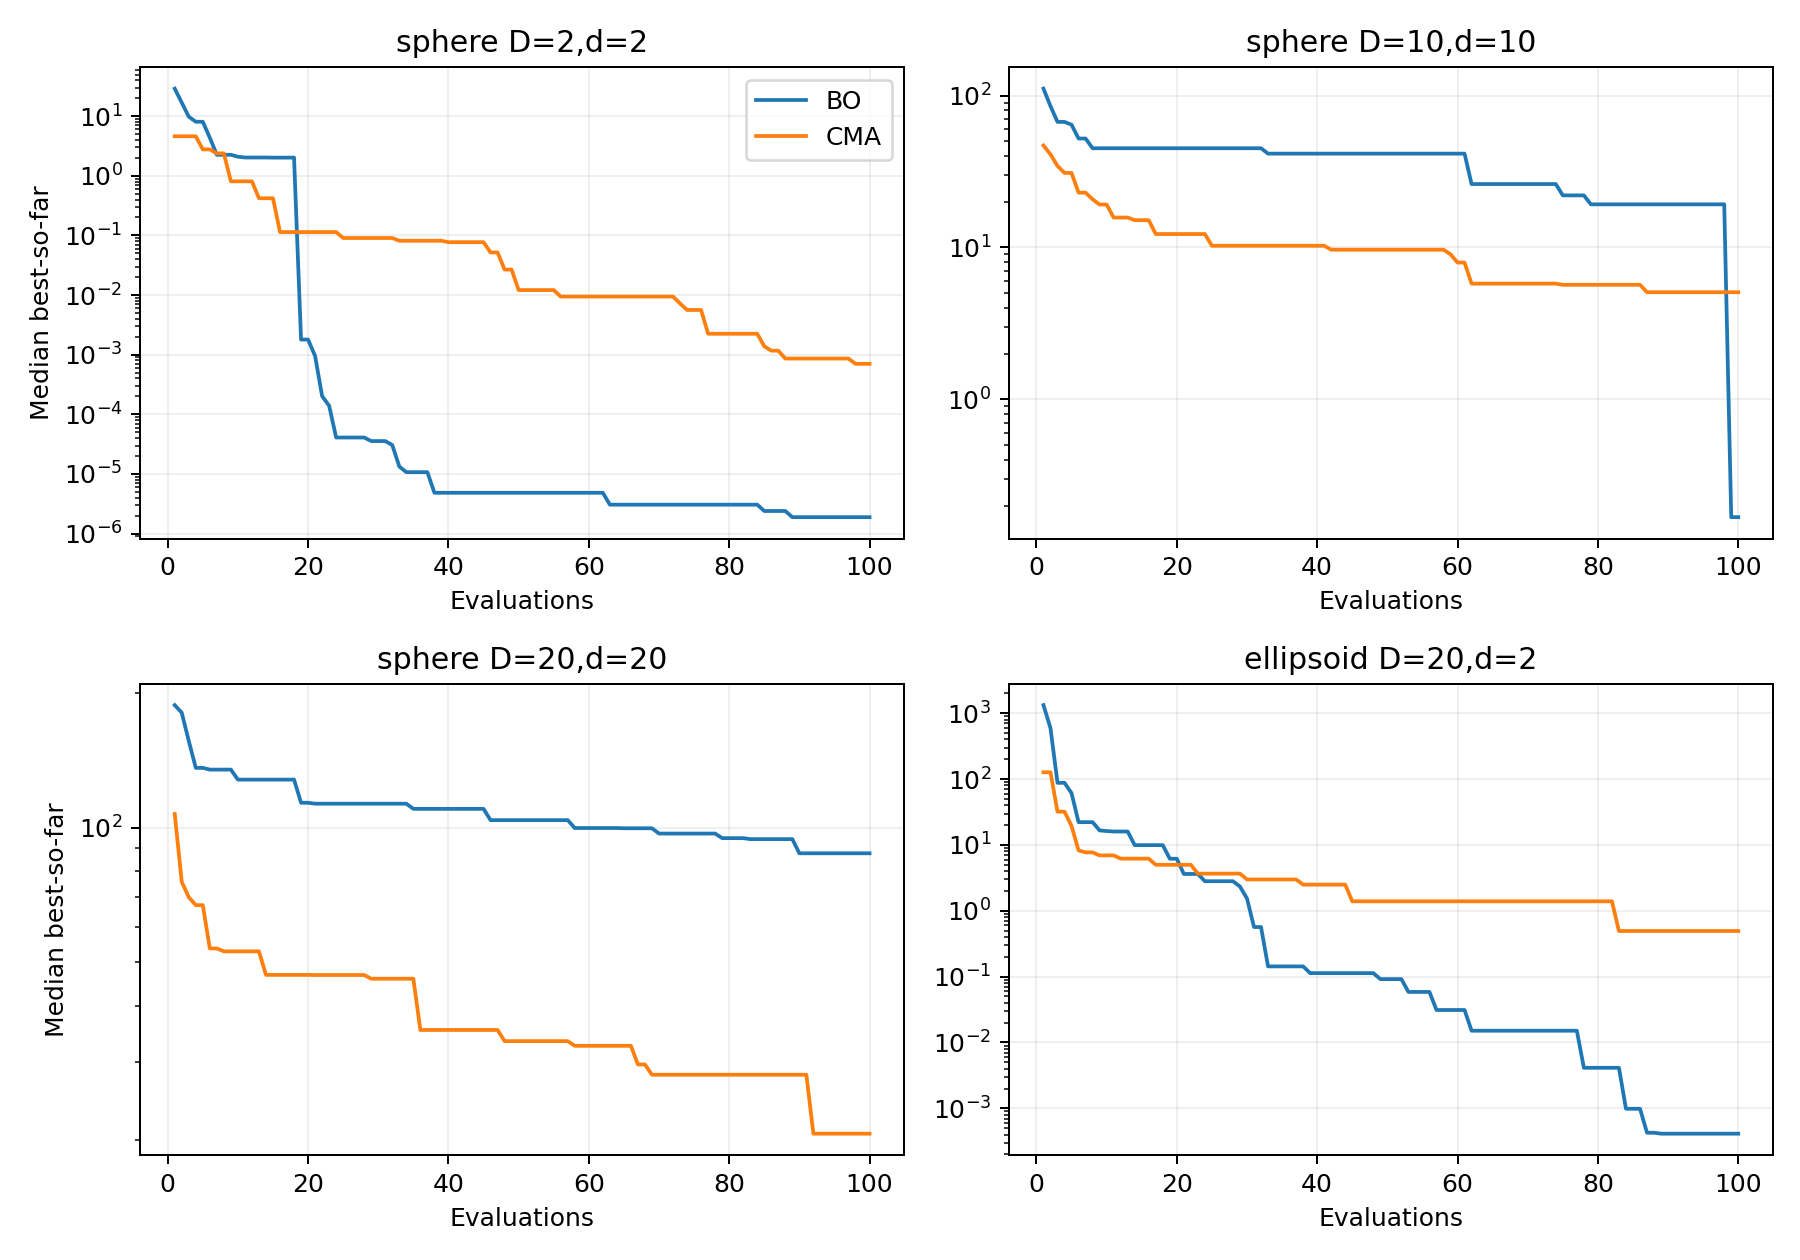
\includegraphics[width=0.9\textwidth]{figures/pilot_convergence.png}
\caption*{Figure 4.1: Median best-so-far over five seeds
(0--4), log scale, budget 100.}
\end{figure}



\begin{figure}[H]
\centering
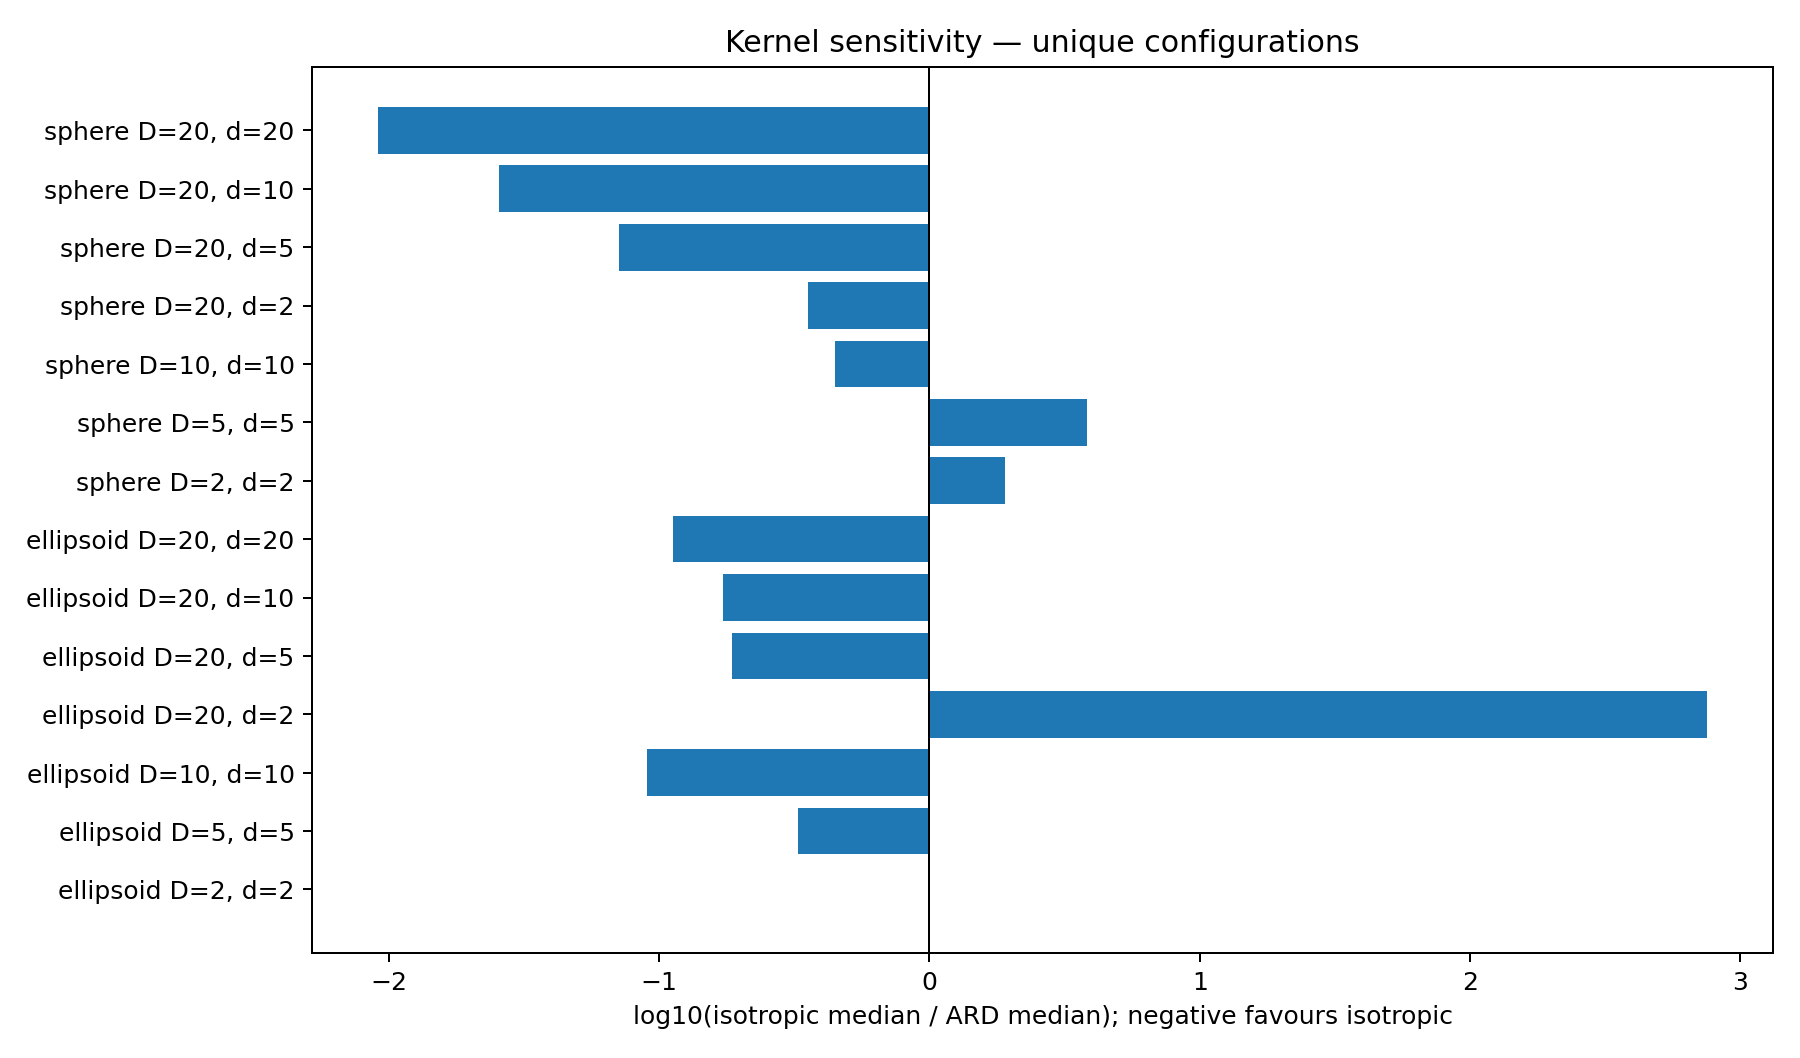
\includegraphics[width=0.9\textwidth]{figures/kernel_sensitivity.png}
\caption*{Figure 4.2: Kernel Sensitivity Comparison}
\end{figure}



\begin{table}[H]
\centering
\caption*{Table 4.1: Median (IQR) final error after
100 evaluations, 10 seeds; BO wins = seeds out of
10 where BO is lower.}
\scriptsize
\setlength{\tabcolsep}{4pt}
\renewcommand{\arraystretch}{1.15}

\begin{tabular}{llccc}
\toprule
\textbf{Obj} &
\textbf{$D,d$} &
\textbf{BO median (IQR)} &
\textbf{CMA-ES median (IQR)} &
\textbf{BO wins} \\
\midrule

Sphere & 2,2 &
$5.6\times10^{-6}$ ($2.0\times10^{-6}$--$1.7\times10^{-5}$) &
$7.0\times10^{-4}$ ($3.1\times10^{-4}$--$9.9\times10^{-4}$) & 10 \\

Sphere & 5,5 &
0.0071 (0.0029--0.024) &
0.34 (0.26--0.47) & 10 \\

Sphere & 10,10 &
11.1 (0.12--25.5) &
4.49 (2.56--6.70) & 5 \\

Sphere & 20,2 &
0.015 ($2.8\times10^{-5}$--0.084) &
0.044 (0.022--0.076) & 5 \\

Sphere & 20,5 &
5.78 (4.25--9.39) &
0.99 (0.77--1.62) & 0 \\

Sphere & 20,10 &
21.6 (5.3--30.4) &
6.09 (4.2--7.4) & 3 \\

Sphere & 20,20 &
87.6 (85.6--95.8) &
23.3 (18.9--25.1) & 0 \\

\midrule

Ellipsoid & 2,2 &
$3.9\times10^{-4}$ ($2.2\times10^{-4}$--0.0011) &
0.013 (0.006--0.036) & 10 \\

Ellipsoid & 5,5 &
0.17 (0.057--0.36) &
3.55 (1.76--4.78) & 9 \\

Ellipsoid & 10,10 &
73 (33--346) &
83 (65--101) & 5 \\

Ellipsoid & 20,2 &
0.008 ($4.2\times10^{-4}$--1.4) &
0.53 (0.42--0.85) & 6 \\

Ellipsoid & 20,5 &
67 (26--101) &
19 (13--29) & 2 \\

Ellipsoid & 20,10 &
357 (230--491) &
137 (81--155) & 2 \\

Ellipsoid & 20,20 &
1182 (901--1558) &
499 (422--535) & 0 \\

\bottomrule
\end{tabular}
\end{table}


%
% === BIBLIOGRAPHY =====
% only if necessary. If your report does not cite any resource,
% which may very well be the case for this assignment, you 
% do not need to add a bibliography
%
\clearpage
\nocite{*}
\bibliographystyle{alpha}
\bibliography{references}


\end{document}



% ----------------------------------------------------------------- %
This document briefly illustrates how you can use Latex to rapidly produce a scientific report. There are many resources online, for example \url{https://www.overleaf.com/learn/latex/Tutorials} With your NUS email, all your team members should be able to join a common Overleaf-project.\\

Here is an example of formula $\int_0^\infty e^{-t} \, dt = 1$ and here is an example of displayed equation,
\begin{align}
\label{eq:proba}
\text{(probability)} = \frac{1}{1 + \exp(-y_i \, \beta^\top x_i)}.
\end{align}
In the above equation $x_i \in \mathbb{R}^p$ is a vector, as well as $\beta \in \mathbb{R}^p$.
This equation describes a logistic regression model. Equation \eqref{eq:proba} has been discussed in the lectures. The following equation
\begin{align}
\label{eq:second_eq}
\iiint e^{-\frac{x^2+y^2+z^2}{2}} \, dx \, dy \, dz = -1
\end{align}
is also interesting. But unfortunately, Equation \eqref{eq:second_eq} is also obviously wrong.
oh

\subsection{How to include images}
Indeed, it is extremely easy to display images. For example, have a look at the Figure \ref{fig:NUS}, it should look familiar.

%
% === EXAMPLE OF DISPLAYED IMAGES ===
%
\begin{figure}[h]
\centering
\includegraphics[width=0.7\textwidth]{example-image}
\caption{a nice plot}
\label{fig:NUS}
\centering
\end{figure}



\subsection{How to cite resources?}
To cite references (eg. articles, book, etc..), it is also extremely easy. For example, a standard textbook describing convex optimization techniques is \cite{boyd2004convex}. You can have a look at \href{https://libguides.usask.ca/c.php?g=218034&p=1445751}{this} to see how to extract citations from Google Scholar and use it in your report. Bibtex is actually very easy to \href{https://www.overleaf.com/learn/latex/Bibliography_management_with_bibtex}{use}.


%
% === BIBLIOGRAPHY =====
% only if necessary. If your report does not cite any resource,
% which may very well be the case for this assignment, you 
% do not need to add a bibliography
%
%\clearpage
\nocite{*}
\bibliographystyle{alpha}
\bibliography{references}


\end{document}
